% Summary schematic of the forms of active control analyzed in the paper.
% Compile standalone:  pdflatex fig_active_processes.tex
% Included in main_revised.tex as fig_active_processes.pdf.
\documentclass[tikz,border=4pt]{standalone}
\usepackage{amssymb}
\usepackage[scaled=0.92]{helvet}
\renewcommand{\familydefault}{\sfdefault}
\usetikzlibrary{arrows.meta,fit,backgrounds,calc}

\definecolor{passive}{HTML}{6B6B6B}
\definecolor{active}{HTML}{D55E00}
\definecolor{panel}{HTML}{F4F4F4}
\definecolor{known}{HTML}{2B7A3D}

\tikzset{
  stage/.style={draw=black!55, rounded corners=3pt, fill=white, minimum width=3.7cm,
                minimum height=4.0cm, inner sep=0pt},
  head/.style={font=\bfseries\small, align=center},
  body/.style={font=\scriptsize, align=left, text width=3.35cm},
  res/.style={font=\scriptsize\itshape, align=left, text width=3.35cm, text=black!80},
  flow/.style={-{Stealth[length=2.6mm]}, line width=0.9pt, black!60},
  scene/.style={draw=black!45, rounded corners=2pt, minimum width=1.25cm, minimum height=0.75cm,
                font=\scriptsize, align=center, fill=white},
}

\newcommand{\kn}[1]{\textcolor{known}{#1\,\checkmark}}
\newcommand{\un}[1]{#1\,?}
\newcommand{\Cv}{\textit{C}}
\hyphenpenalty=10000 \exhyphenpenalty=10000

\begin{document}
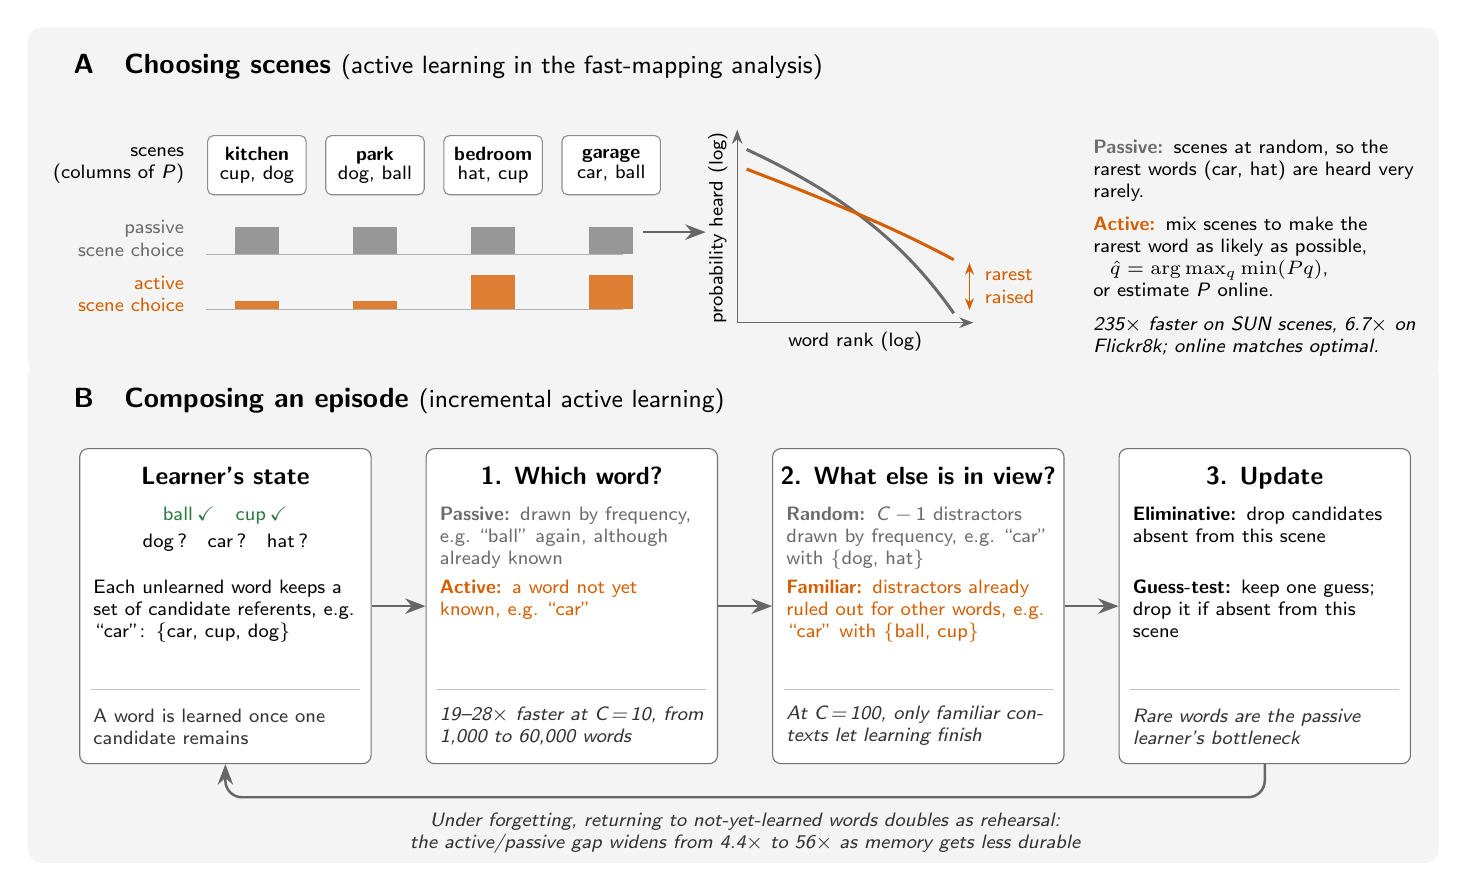
\begin{tikzpicture}

% =====================================================================
% Panel A: choosing scenes (fast-mapping analysis)
% =====================================================================
\node[font=\bfseries, anchor=west] (Atitle) at (0, 9.0)
  {A\quad Choosing scenes \normalfont\small(active learning in the fast-mapping analysis)};

% left labels
\node[font=\scriptsize, anchor=east, align=right] at (1.65, 7.75) {scenes\\(columns of \textit{P})};
\node[font=\scriptsize, text=passive, anchor=east, align=right] at (1.65, 6.82) {passive\\scene choice};
\node[font=\scriptsize, text=active, anchor=east, align=right] at (1.65, 6.12) {active\\scene choice};

% four scenes and their choice weights
\foreach \i/\nm/\objs in {0/kitchen/{cup, dog}, 1/park/{dog, ball}, 2/bedroom/{hat, cup}, 3/garage/{car, ball}} {
  \node[scene] (s\i) at (2.45 + 1.5*\i, 7.75) {\textbf{\nm}\\[-1pt]\objs};
}
\foreach \i/\hp/\ha in {0/0.34/0.10, 1/0.34/0.10, 2/0.34/0.44, 3/0.34/0.44} {
  \fill[passive!70] (2.17 + 1.5*\i, 6.62) rectangle ++(0.56, \hp);
  \fill[active!80]  (2.17 + 1.5*\i, 5.92) rectangle ++(0.56, \ha);
}
\draw[black!30] (1.8, 6.62) -- (7.1, 6.62);
\draw[black!30] (1.8, 5.92) -- (7.1, 5.92);

\draw[flow] (7.35, 6.9) -- (8.15, 6.9);

% resulting word-referent distribution (schematic rank-frequency, log-log)
\begin{scope}[shift={(8.55, 5.75)}]
  \draw[-{Stealth[length=1.8mm]}, black!60] (0,0) -- (3.0,0);
  \draw[-{Stealth[length=1.8mm]}, black!60] (0,0) -- (0,2.45);
  \node[font=\scriptsize, anchor=north] at (1.5,0) {word rank (log)};
  \node[font=\scriptsize, rotate=90, anchor=south] at (0,1.2) {probability heard (log)};
  \draw[passive, line width=1.1pt] (0.12,2.2) .. controls (1.3,1.65) and (2.1,1.05) .. (2.75,0.12);
  \draw[active, line width=1.1pt]  (0.12,1.95) .. controls (1.3,1.5) and (2.1,1.15) .. (2.75,0.8);
  \draw[{Stealth[length=1.5mm]}-{Stealth[length=1.5mm]}, active, line width=0.7pt] (2.95,0.16) -- (2.95,0.76);
  \node[font=\scriptsize, text=active, anchor=west, align=left] at (3.02,0.46) {rarest\\raised};
\end{scope}

% explanation column
\node[font=\scriptsize, align=left, anchor=north west, text width=4.15cm] at (12.95, 8.2) {
  \textcolor{passive}{\textbf{Passive:}} scenes at random, so the rarest words (car, hat) are heard very rarely.\\[4pt]
  \textcolor{active}{\textbf{Active:}} mix scenes to make the rarest word as likely as possible,\\
  \hspace*{0.8em}$\hat q = \arg\max_q \min(Pq)$,\\
  or estimate \textit{P} online.\\[4pt]
  \textit{235$\times$ faster on SUN scenes, 6.7$\times$ on Flickr8k; online matches optimal.}};

\begin{scope}[on background layer]
  \node[fill=panel, rounded corners=5pt, fit={(Atitle) (-0.25,5.3) (17.25,8.3)}, inner sep=6pt] {};
\end{scope}

% =====================================================================
% Panel B: composing an episode (incremental learners)
% =====================================================================
\node[font=\bfseries, anchor=west] (Btitle) at (0, 4.75)
  {B\quad Composing an episode \normalfont\small(incremental active learning)};

\node[stage] (state)   at (2.05, 2.15) {};
\node[stage] (target)  at (6.45, 2.15) {};
\node[stage] (context) at (10.85, 2.15) {};
\node[stage] (update)  at (15.25, 2.15) {};

% rule separating each box's result line
\foreach \b in {state, target, context, update} {
  \draw[black!25] ($(\b.south west)+(0.15,0.95)$) -- ($(\b.south east)+(-0.15,0.95)$);
}

% --- learner state
\node[head, anchor=north] at ([yshift=-0.12cm]state.north) {Learner's state};
\node[font=\scriptsize, align=center, anchor=north] at ([yshift=-0.62cm]state.north)
  {\kn{ball}\quad \kn{cup}\\[2pt] \un{dog}\quad \un{car}\quad \un{hat}};
\node[body, anchor=north] at ([yshift=-1.55cm]state.north)
  {Each unlearned word keeps a set of candidate referents, e.g.\ ``car'': \{car, cup, dog\}};
\node[res, anchor=south] at ([yshift=0.12cm]state.south)
  {\upshape A word is learned once one candidate remains};

% --- target selection
\node[head, anchor=north] at ([yshift=-0.12cm]target.north) {1. Which word?};
\node[body, text=passive, anchor=north] at ([yshift=-0.62cm]target.north)
  {\textbf{Passive:} drawn by frequency, e.g.\ ``ball'' again, although already known};
\node[body, text=active, anchor=north] at ([yshift=-1.55cm]target.north)
  {\textbf{Active:} a word not yet known, e.g.\ ``car''};
\node[res, anchor=south] at ([yshift=0.12cm]target.south)
  {19--28$\times$ faster at \Cv\,=\,10, from 1,000 to 60,000 words};

% --- context selection
\node[head, anchor=north] at ([yshift=-0.12cm]context.north) {2. What else is in view?};
\node[body, text=passive, anchor=north] at ([yshift=-0.62cm]context.north)
  {\textbf{Random:} \Cv$\,-\,$1 distractors drawn by frequency, e.g.\ ``car'' with \{dog, hat\}};
\node[body, text=active, anchor=north] at ([yshift=-1.55cm]context.north)
  {\textbf{Familiar:} distractors already ruled out for other words, e.g.\ ``car'' with \{ball, cup\}};
\node[res, anchor=south] at ([yshift=0.12cm]context.south)
  {At \Cv\,=\,100, only familiar contexts let learning finish};

% --- update
\node[head, anchor=north] at ([yshift=-0.12cm]update.north) {3. Update};
\node[body, anchor=north] at ([yshift=-0.62cm]update.north)
  {\textbf{Eliminative:} drop candidates absent from this scene};
\node[body, anchor=north] at ([yshift=-1.55cm]update.north)
  {\textbf{Guess-test:} keep one guess; drop it if absent from this scene};
\node[res, anchor=south] at ([yshift=0.12cm]update.south)
  {Rare words are the passive learner's bottleneck};

% flow arrows and loop
\draw[flow] (state.east) -- (target.west);
\draw[flow] (target.east) -- (context.west);
\draw[flow] (context.east) -- (update.west);
\draw[flow, rounded corners=6pt] (update.south) -- ++(0,-0.42) -| (state.south);
\node[font=\scriptsize\itshape, align=center, text width=10cm, text=black!80, anchor=north]
  at ($(state.south)!0.5!(update.south) + (0,-0.5)$)
  {Under forgetting, returning to not-yet-learned words doubles as rehearsal:\\
   the active/passive gap widens from 4.4$\times$ to 56$\times$ as memory gets less durable};

\begin{scope}[on background layer]
  \node[fill=panel, rounded corners=5pt, fit={(Btitle) (-0.25,-0.9) (17.25,0)}, inner sep=6pt] {};
\end{scope}

\end{tikzpicture}
\end{document}
